\documentclass{standalone}

\usepackage{tikz}

\begin{document}

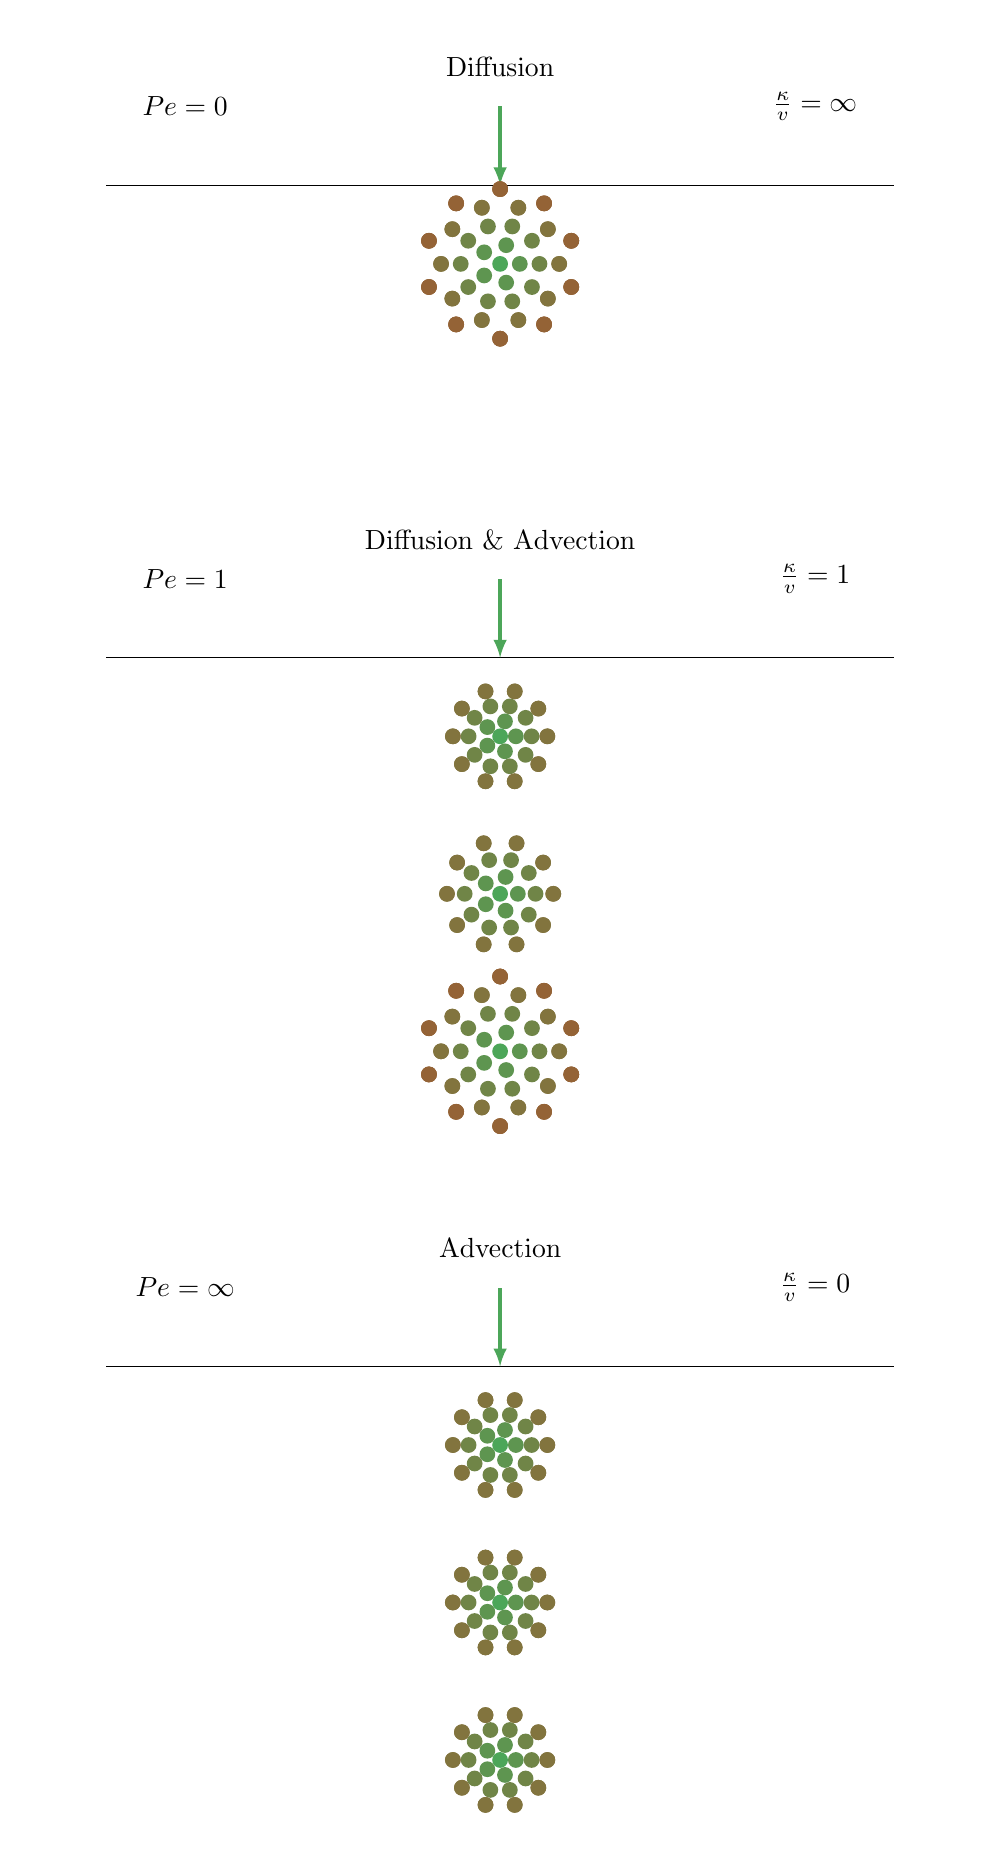
\begin{tikzpicture}
%\fill[fill=gray!50!yellow!10] (-6,-21) rectangle (6,2);
\fill[fill=white] (-6,-21) rectangle (6,2);

\draw (0,1.5) node {Diffusion};

\draw (-4,1) node {$Pe = 0$};
\draw (4, 1) node {$\frac{\kappa}{v} = \infty$};

%\draw[white] (0,0) circle (6) ;
\draw (-5,0) -- (5,0) ;
\draw[very thick, teal!70!yellow] [latex-] (0,0) -- (0,1) ;
\fill[teal!70!yellow] (0, -1) circle (0.1) ;

\foreach \x in{1,...,5}
\fill[teal!70!yellow!90!red] (0, -1) ++(\x *72:0.25) circle (0.1) ;

\foreach \x in{1,...,10}
\fill[teal!70!yellow!80!red] (0, -1) ++(\x * 36:0.5) circle (0.1) ;

\foreach \x in {1,...,20}
\fill[teal!70!yellow!70!red] (0, -1) ++(\x * 36:0.75) circle (0.1) ;

\foreach \x in{1,...,30}
\fill[teal!70!yellow!60!red] (0, -1) ++(\x *36+18:0.95) circle (0.1) ;

%%%
\draw (0,-4.5) node {Diffusion \& Advection};
\draw (-4,-5) node {$Pe = 1$};
\draw (4, -5) node {$\frac{\kappa}{v} = 1$};

\draw (-5,-6) -- (5,-6) ;
\draw[very thick, teal!70!yellow] [latex-] (0,-6) -- (0,-5) ;
\fill[teal!70!yellow] (0, -7) circle (0.1) ;

\foreach \x in{1,...,5}
\fill[teal!70!yellow!90!red] (0, -7) ++(\x *72:0.2) circle (0.1) ;

\foreach \x in{1,...,10}
\fill[teal!70!yellow!80!red] (0, -7) ++(\x * 36:0.4) circle (0.1) ;

\foreach \x in {1,...,20}
\fill[teal!70!yellow!70!red] (0, -7) ++(\x * 36:0.6) circle (0.1) ;

\fill[teal!70!yellow] (0, -9) circle (0.1) ;
\foreach \x in{1,...,5}
\fill[teal!70!yellow!90!red] (0, -9) ++(\x *72:0.225) circle (0.1) ;

\foreach \x in{1,...,10}
\fill[teal!70!yellow!80!red] (0, -9) ++(\x * 36:0.45) circle (0.1) ;

\foreach \x in {1,...,20}
\fill[teal!70!yellow!70!red] (0, -9) ++(\x * 36:0.675) circle (0.1) ;

\fill[teal!70!yellow] (0, -11) circle (0.1) ;
\foreach \x in{1,...,5}
\fill[teal!70!yellow!90!red] (0, -11) ++(\x *72:0.25) circle (0.1) ;

\foreach \x in{1,...,10}
\fill[teal!70!yellow!80!red] (0, -11) ++(\x * 36:0.5) circle (0.1) ;

\foreach \x in {1,...,20}
\fill[teal!70!yellow!70!red] (0, -11) ++(\x * 36:0.75) circle (0.1) ;

\foreach \x in{1,...,30}
\fill[teal!70!yellow!60!red] (0, -11) ++(\x *36+18:0.95) circle (0.1) ;

%%%
\draw (0,-13.5) node {Advection};
\draw (-4,-14) node {$Pe = \infty$};
\draw (4, -14) node {$\frac{\kappa}{v} = 0$};

\draw (-5,-15) -- (5,-15) ;
\draw[very thick, teal!70!yellow] [latex-] (0,-15) -- (0,-14) ;
\fill[teal!70!yellow] (0, -16) circle (0.1) ;

\foreach \x in{1,...,5}
\fill[teal!70!yellow!90!red] (0, -16) ++(\x *72:0.2) circle (0.1) ;

\foreach \x in{1,...,10}
\fill[teal!70!yellow!80!red] (0, -16) ++(\x * 36:0.4) circle (0.1) ;

\foreach \x in {1,...,20}
\fill[teal!70!yellow!70!red] (0, -16) ++(\x * 36:0.6) circle (0.1) ;


\fill[teal!70!yellow] (0, -18) circle (0.1) ;
\foreach \x in{1,...,5}
\fill[teal!70!yellow!90!red] (0, -18) ++(\x *72:0.2) circle (0.1) ;

\foreach \x in{1,...,10}
\fill[teal!70!yellow!80!red] (0, -18) ++(\x * 36:0.4) circle (0.1) ;

\foreach \x in {1,...,20}
\fill[teal!70!yellow!70!red] (0, -18) ++(\x * 36:0.6) circle (0.1) ;

\fill[teal!70!yellow] (0, -20) circle (0.1) ;
\foreach \x in{1,...,5}
\fill[teal!70!yellow!90!red] (0, -20) ++(\x *72:0.2) circle (0.1) ;

\foreach \x in{1,...,10}
\fill[teal!70!yellow!80!red] (0, -20) ++(\x * 36:0.4) circle (0.1) ;

\foreach \x in {1,...,20}
\fill[teal!70!yellow!70!red] (0, -20) ++(\x * 36:0.6) circle (0.1) ;

\end{tikzpicture}

\end{document}